\documentclass[letterpaper,12pt]{article}
\usepackage[utf8]{inputenc}
\usepackage[T1]{fontenc}
\usepackage{charter} %%%font
\usepackage[spanish]{babel}
\usepackage{charter}
\usepackage{geometry}
\usepackage{amsmath}
\usepackage{float}
\usepackage{graphicx}
\usepackage{subcaption}
\usepackage{amssymb}
\usepackage{adjustbox}
\usepackage{wrapfig} 
\usepackage{xcolor}
\usepackage{fancyhdr}
\usepackage{biblatex}
\usepackage{tabularx}
\usepackage{fancyhdr}
\usepackage{comment}

%%%%%%%%%CODIGO FUENTE PARA DOCUMENTO
\thispagestyle{empty}
\title{title} 
\author{asd}
\geometry{top=2cm, bottom=2cm, left=2cm, right= 2cm} %%margen
\graphicspath{{images/}}

\begin{document}
\maketitle
\thispagestyle{empty}
\newpage
\thispagestyle{empty}
\tableofcontents %%%%%%%%%%%%%%%%%%%%%%
\newpage
\setcounter{page}{1}
\pagestyle{headings}

\begin{sloppypar}
\section{Introducción}
Poco se habla de las repercusiones que pueden tener al estar dentro de los hogares o en los basureros convencionales, gran parte de los componentes electrónicos que se encuentran en los hogares (computadoras, teléfonos móviles,electrodomésticos y/o televisores) contienen sustancias toxicas y volátiles como mercurio y cadmio, entre otros de las cuales, en su gran mayoría, desconocen las personas encargadas del hogar. Una larga exposición a estas sustancias (y dependiendo de que sustancia se hable) puede generar problemas en la salud tales como cáncer, cardiopatías, afectaciones a los fetos etc. En el medio ambiente, la mala gestión de estos desechos contamina la atmósfera y los cuerpos de agua de los que nos abastecemos para el uso cotidiano.

Este hecho es realmente alarmante si nos cuestionamos sobre el rápido avance tecnológico alrededor del mundo, el uso de equipos electrónicos se ha vuelto cada vez más frecuente y, por lo tanto, aumentan las cifras sobre la basura tecnológica. México no es la excepción ya que alrededor de 300 mil toneladas pertenecientes a desechos electrónicos tienen como destino final los basureros municipales o rellenos sanitarios, teniendo un estimado de 170 mil toneladas pertenecientes solamente a televisiones análogas. (Desechos electrónicos y alternativas al ambiente, 2022)
\newpage
\section{Fenómeno a Estudiar}
\subsection{Planteamiento del problema}
Hoy en día en Veracruz la mayoría de las personas tiene a la mano cualquier dispositivo electrónico, desde un teléfono o hasta una computadora, a consecuencia de este hecho existe una gran desmedida de aparatos electrónicos que ha contribuido a un alto aumento de “basura tecnológica” en el estado y en todo el mundo. En la región, cada cuatrimestre se tiene alrededor de 20 toneladas de basura tecnológica entre pantallas, bocinas y teléfonos celulares (Periodistasdigitales, 2022). 

Poco se habla de las consecuencias que pueden traer consigo la basura tecnológica al estar en contacto con las personas y el medio ambiente sin un manejo apropiado. No toda la población conoce que se usan ciertos metales y sustancias toxicas para la fabricación de aparatos electrónicos con los que convivimos en nuestra vida cotidiana en los hogares; Veracruz también refleja la situación del país en cuanto a la basura electrónica; es decir, se desconoce la producción y el desecho de productos electrónicos en la entidad.
\vspace{0.3cm}\\ 
Se cree que se generan altos niveles de contaminación, pero son difíciles de cuantificar, por lo que es necesario sumar esfuerzos para entender y abordar el problema actual y potencial de la generación y el manejo de la basura electrónica, que van en aumento. En nuestro país la cultura de reciclaje es muy pobre, por lo que es realmente importante impulsar a los ciudadanos a promover el reciclaje de la basura tecnológica y tratar de consumir dichos aparatos con responsabilidad.
\begin{figure}[H]
    \centering 
    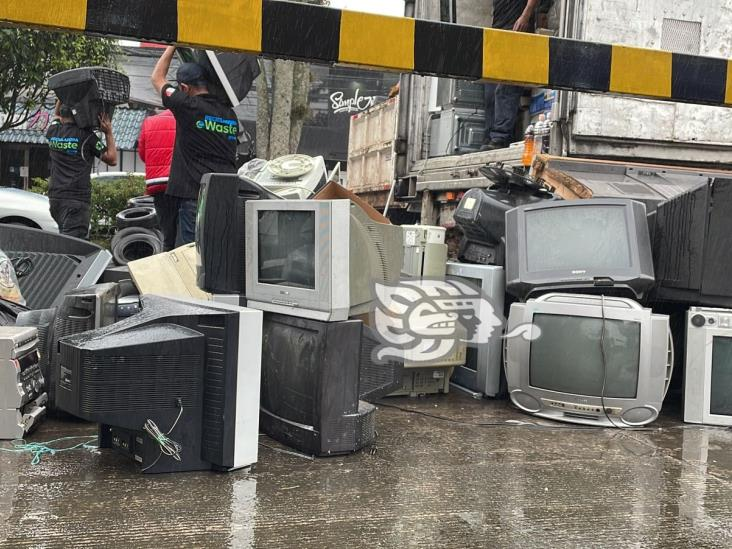
\includegraphics[width = 0.8 \linewidth]{basura.jpg}
\end{figure}

\newpage
\section{¿Cómo afecta la basura tecnológica en la salud?}
La basura tecnológica o RAEE (residuos de aparatos electrónicos y eléctricos), se define como todo dispositivo alimentado con energía eléctrica cuya vida útil termina (Iberdrola, 2019), por ejemplo, teléfonos celulares, equipos de cómputo, congeladores, televisores, impresoras, electrodomésticos, equipos de sonido, secadoras de cabello, planchas, cepillos dentales eléctricos, tabletas etc. Los riesgos que estos desechos electrónicos representan para la salud son inminentes debido al alto contenido de materiales tóxicos que, al combinarse con la lluvia y otras sustancias, se convierten en agentes tóxicos para el agua, aire, suelo y personas que convergen alrededor de ellos. (Desechos electrónicos y alternativas al ambiente, 2022). Los desechos electrónicos se acumulan en los vertederos de todo el mundo, filtrando sustancias peligrosas al medio ambiente y la salud.
\vspace{0.3cm}\\ 
Según el Programa para el Medio Ambiente de las Naciones Unidas, se generan cerca de 50 millones de toneladas de desechos electrónicos al año. Y la mayoría no pasan por el sistema de reciclaje óptimo para el medio ambiente. (Bilbao, 2022). 

En México, cada año se generan más de 1.1. millones de toneladas de residuos eléctricos y electrónicos, 6\% de ellos cuentan con materiales altamente contaminantes como: metales pesados, baterías y plásticos con retardantes de flama que pueden provocar graves daños a la salud y el medio ambiente (Del Consumidor, P. F., 2021)

\section{Contaminación por basura tecnológica en Veracruz}
En los últimos 4 años, aumentó un 75\% los desechos de celulares, tabletas y pantallas electrónicas, unas cinco toneladas de basura tecnológica mensuales se generan en el
estado de Veracruz, cantidad que tiende a incrementarse conforme avanza la tecnología y muchos aparatos son desechados al no poder actualizarse. (Noticias desde Veracruz,
2022)
\vspace{0.3cm}\\ 
De acuerdo con grupos ambientalistas e instancias como la Secretaría de Medio Ambiente, dichos componentes ponen en riesgo al ecosistema del estado ya que, además de tardar mucho tiempo en degradarse, generan importantes índices de contaminación. Con más de 8 millones de habitantes en los 212 municipios, en Veracruz solo operan seis rellenos sanitarios de manera eficiente, y la mayor parte de los desechos que se generan son depositados en basureros a cielo abierto. Los problemas de contaminación ambiental que generan más de 6 mil toneladas diarias de basura no han podido ser resueltos, pues administraciones municipales y estatales vienen y van, sin invertir en la solución.
\vspace{0.3cm}\\ 
Tampoco han servido de nada las clausuras de basureros y rellenos sanitarios que no cumplen con su función. Las promesas de sanear los tiraderos han sido banderas políticas
muy recurridas, pues una vez en los cargos los funcionarios se olvidan de ellas (Zamudio, 2022).
\newpage
\section{Datos a obtener}

\begin{itemize}
    \item \textbf{Cantidad de Basura Tecnológica:} Se menciona que cada cuatrimestre se generan alrededor de 20 toneladas de basura tecnológica en la región. Podrías recopilar datos históricos sobre la cantidad de basura tecnológica generada en Veracruz durante varios años para analizar tendencias y proyecciones futuras.
    \item \textbf{Tasa de Obsolescencia de Dispositivos Electrónicos:} Se afirma que los dispositivos electrónicos y eléctricos son obsoletos en pocos años de uso. Sería interesante recopilar datos sobre la tasa de obsolescencia de diferentes tipos de dispositivos electrónicos, como teléfonos celulares, computadoras, televisores, etc., para comprender mejor este fenómeno.
    \item \textbf{Comportamiento de Consumo de la Población:} Se sugiere que, a pesar de tener acceso a información sobre la basura tecnológica, la población sigue consumiendo dispositivos electrónicos de manera indiscriminada. Sería útil recopilar datos sobre el comportamiento de consumo de la población en relación con los dispositivos electrónicos y su disposición adecuada.
    \item \textbf{Impacto Ambiental de la Basura Tecnológica:} Se menciona que la basura tecnológica puede tener consecuencias ambientales graves. Podrías recopilar datos sobre el impacto ambiental de la basura tecnológica en términos de contaminación del suelo, agua y aire, así como su efecto en la biodiversidad local.
    \item \textbf{Participación en Programas de Reciclaje:} Dado que se menciona que la cultura de reciclaje es pobre en el país, podrías recopilar datos sobre la participación de la población en programas de reciclaje de basura tecnológica, como la cantidad de dispositivos electrónicos recolectados y reciclados en comparación con la cantidad total de desechos electrónicos generados.
\end{itemize}
\subsection{Hipótesis}
La población no está consciente de esta problemática que crece al mismo tiempo que los avances tecnológicos, los dispositivos electrónicos y eléctricos son obsoletos en pocos años de uso y son cambiados constantemente por modelos más recientes y modernos, acelerando el número de basura tecnológica. Existe información amplia que nos describe las consecuencias que actualmente está causando la basura tecnológica y los estragos que puede traer a futuro si no se toma acción ante este problema; la población, incluso aunque disponga de esta información con unos pocos clics, prefiere vivir en la ignorancia haciendo de lado los problemas que nos afectan como sociedad y, a pesar de que estén enterados de dicha problemática, no dejan de caer en la misma rutina y mantienen indiferencia dentro del tema, lo que causa más basura.
\newpage
\section{Distribución de los datos}
\subsection{Población y Muestra}
Para determinar el tipo de muestreo más adecuado para la población que se va a estudiar, es importante considerar varios factores, como la accesibilidad de la población, el tamaño de la muestra requerida, el presupuesto disponible y la representatividad de la muestra. Dado el contexto del estudio sobre el reciclaje de basura tecnológica en Veracruz, podríamos considerar diferentes enfoques de muestreo: 
\begin{itemize}
    \item Variable Independiente: Exposición a la campaña de concientización sobre el reciclaje de basura tecnológica.
    \item Espacio Muestral: Ciudadanos de Veracruz mayores de 13 años.
\end{itemize}
Dentro de nuestro ámbito de estudio se encuentran los ciudadanos de Veracruz, teniendo
una población de 8,062,579 habitantes, es decir, el 6.4\% del total del país. (INEGI, 2020)
\vspace{0.3cm}\\
Para calcular nuestra muestra, se utilizó la siguiente fórmula:
$$ n = \frac{Z^{2}p(1-p)}{E^{2}}$$
Donde:
\begin{itemize}
    \item $n$ es el tamaño de la muestra
    \item $Z$ es el valor crítico de la distribución normal estándar relacionado con el nivel de confianza.
    \item $p$ es la estimación de la proporción de la población.
    \item $E$ es el margen de error.
\end{itemize}
Se decide por un nivel de confianza del 95\%, un margen de error del 10\% y 0.5 como valor estándar para la proporción de la población. Para obtener Z con el 95\% de nivel de confianza se calcularon los siguientes datos a través de la siguiente tabla:

\begin{center}
    \begin{tabular}[H]{|c|c|c|}\hline
        Nivel de confianza \% & Nivel de significancia $\alpha$ & $Z = 1 - \frac{\alpha}{2}$ \\  \hline
        95\% & $ \alpha a 1 - 0.95 = 0.05$ & $1 - \frac{0.05}{2} = 0.975$ \\ \hline
    \end{tabular}
\end{center}
Para calcular el valor crítico de Z se debe de consultar la tabla de distribución normal estándar (mejor conocida como tabla Z), correspondiente al área bajo la curva de la distribución normal. De acuerdo dicha tabla, el valor de Z es 1.96.
\vspace{0.3cm}\\ 
Calculando la muestra nos arroja un resultado de:
$$ n = \frac{{1.96}^{2}0.5(1-0.5)}{{0.10}^{2}} = 96.04$$
El tamaño arrojado se redondea hacia arriba a 97 dado que la muestra siempre debe ser un número entero.

\section{Distribución de datos}
\subsection{Variables aleatorias}
La distribución de los datos en este caso estaría influenciada por el comportamiento de los ciudadanos con respecto al reciclaje de basura tecnológica antes y después de la campaña de concientización. Podemos esperar que la distribución de los datos refleje diferentes patrones de comportamiento entre los grupos experimental y de control.
\vspace{0.3cm}\\
Además, la distribución de los datos también puede verse afectada por otros factores, como la demografía de la población de Veracruz, la disponibilidad de instalaciones de reciclaje, el nivel de conciencia ambiental de los ciudadanos, entre otros. Es importante tener en cuenta estos factores al interpretar la distribución de los datos y sacar conclusiones sobre el impacto de la campaña de concientización sobre el reciclaje de basura tecnológica.
\vspace{0.3cm}\\ 
Se puede considerar:
\begin{enumerate}
    \item Edad 
    \item Nivel de educación
    \item Comportamiento de reciclaje
    \item Acceso a instalaciones de reciclaje
\end{enumerate}
\section{Estudio del fenómeno}
\subsection{Elementos de la Probabilidad y Estadística útiles}
En el estudio del fenómeno del reciclaje de basura tecnológica en Veracruz, los principios de la probabilidad y la estadística son fundamentales para analizar y comprender diversos aspectos del comportamiento ciudadano y el impacto de las intervenciones. Estas disciplinas ofrecen herramientas valiosas para examinar la frecuencia de ciertos comportamientos de reciclaje, identificar patrones y tendencias, así como caracterizar el comportamiento promedio y la variabilidad en la participación ciudadana en el reciclaje. Además, permiten comparar tasas de reciclaje entre diferentes grupos, evaluar la efectividad de las campañas de concientización y otras intervenciones, e identificar factores que influyen en el comportamiento de reciclaje, como variables demográficas o socioeconómicas. En conjunto, estos enfoques proporcionan una base sólida para abordar el fenómeno del reciclaje de basura tecnológica en Veracruz.
\begin{itemize}
    \item Probabilidad: que un ciudadano de Veracruz recicle adecuadamente su basura tecnológica, que participe en programas de reciclaje o que tenga acceso a instalaciones.
    \item Inferencia estadística: Estimar la proporción de ciudadanos en Veracruz que reciclan su basura tecnológica utilizando una muestra representativa o si existe una relación significativa entre el nivel educativo y la participación en programas de reciclaje en Veracruz.
    \item Estimación Puntual: Estimar la proporción de ciudadanos en Veracruz que reciclan su basura tecnológica a partir de una encuesta realizada a una muestra de la población, la media de la cantidad de basura tecnológica reciclada por hogar en Veracruz utilizando datos recopilados de puntos de reciclaje y la proporción de ciudadanos en Veracruz que conocen las políticas de reciclaje de basura tecnológica a partir de datos administrativos.
    \item Estimación de intervalo: Determinar un intervalo de confianza para la media de la cantidad de basura tecnológica reciclada por hogar en Veracruz basado en datos de reciclaje recolectados durante un período de tiempo específico.
    \item Prueba de hipótesis: Probar si existe una diferencia significativa en la cantidad de basura tecnológica reciclada entre ciudadanos con acceso a instalaciones de reciclaje y aquellos sin acceso o si el nivel educativo tiene un efecto significativo en la participación en programas de reciclaje de basura tecnológica en Veracruz.
\end{itemize}
\begin{figure}[H]
    \centering 
    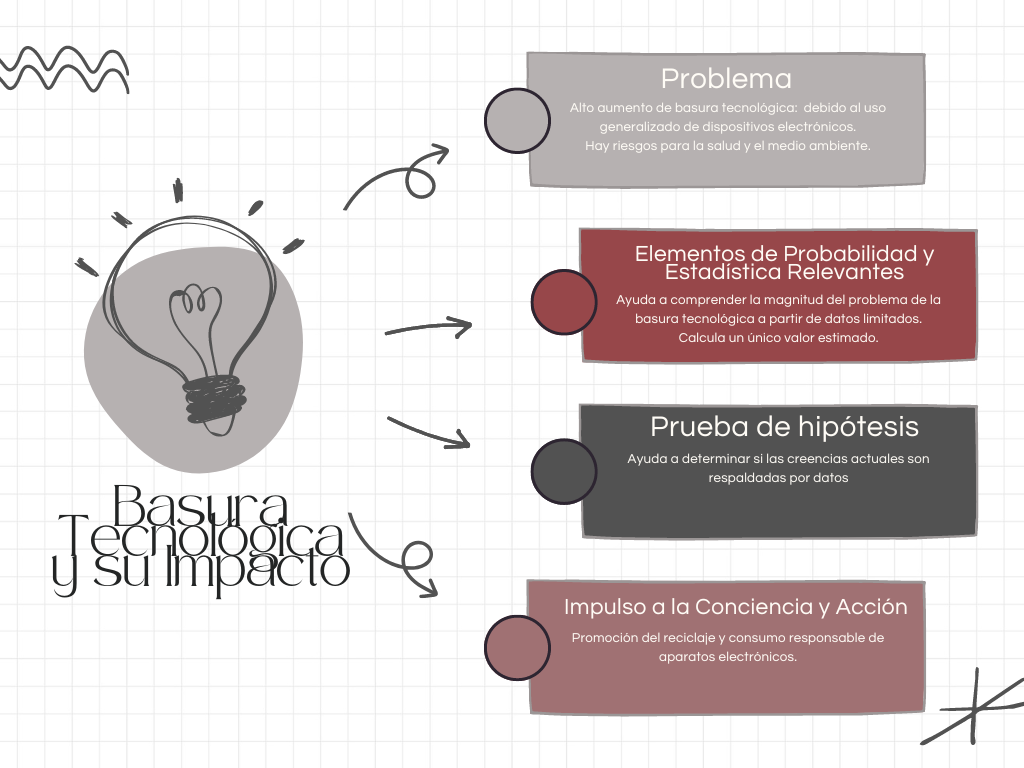
\includegraphics[width = 0.8 \linewidth]{mapa.png}
\end{figure}

\end{sloppypar}

\newpage

\begin{thebibliography}{9}  
\bibitem{1}
Universidad Veracruzana. Dirección de Comunicación de la Ciencia. 
\emph{Desechos electrónicos y alternativas al ambiente.} (2022).
\url{https://www.uv.mx/cienciauv/blog/desechoselectronicosyalternativasalambiente/} 

\bibitem{2}
Redbioética/UNESCO, \emph{Basura electrónica: amenaza a la salud}, (2021). 
\url{https://\redbioetica.com.ar/basura-electronica-amenaza-a-la-salud/}

\bibitem{3}
Gobierno de México. \emph{Recicla tus dispositivos.} Del Consumidor, P. F. (2021). 
\url{https://www.gob.mx/profeco/es/articulos/recicla-tus-dispositivos?idiom=es}

\bibitem{4}
\emph{La basura electrónica y su peligro para el medio ambiente. } Flores, J. (2023).
\url{https://www.nationalgeographic.com.es/mundo-ng/peligros-basura-electronica_13239}

\bibitem{5}
INEGI. \emph{Resumen.} Veracruz, 2020.
\url{https://cuentame.inegi.org.mx/monografias/informacion/ver/}

\bibitem{6}
Periodistasdigitales. \emph{Hasta 20 toneladas de basura tecnológica en el estado de Veracruz.} Plumas libres. 2022.

\bibitem{7}
\emph{Introducción a la probabilidad y estadística.} William Mendenhall, Robert J. Beaver y Barbara M. Beaver.

\bibitem{8}
\emph{Probabilidad y estadística.} Murray R. Spiegel.


\end{thebibliography}
\end{document}